\chapter{Studying cities}
\label{chap:studying_cities}

\begin{flushright}{\slshape    
Chaos was the law of nature;\\
Order was the dream of man.} \\ \medskip
--- Henry Adams~\cite{Adams:1990}
\end{flushright}

\bigskip

Cities appeared some $10,000$ years ago~\cite{Bairoch:1985, Mumford:1961}
concomitantly with the agriculture revolution, and really started to
thrive after the industrial revolution~\cite{Bairoch:1985}.  In England first,
where the revolution was born; London was the first city in the modern world
to reach $1,000,000$ inhabitants at the beginning of the $19$th century. The
urban growth then slowly spread through the end of the $19$th and the $20$th to
the rest of the Western world. Now, while western countries are already
mostly urban (as of $2014$, the United States' population was $82\%$ urban,
Japan's cities hosted $93\%$ of the population, and most countries in the European Union were around the $80\%$
mark), most of what has been dubbed the 'urban \graffito{Source:\\ UN Population
Division (2011)} revolution' is happening in developing countries. A symbolic
barrier was reached in $2005$, when it was estimated by the U.N. that more than
$50\%$ of the world total population was living in cities. It is not difficult
to convince oneself that urbanisation is not an accident in human history, and
that cities' influence and impact are not going to stop growing any time soon.

In fact, the impact of cities is already tremendous. First, they have a
disproportionately large importance in the world's economy. A 2012 report by
McKinsey noted that while cities represented respectively $79\%$ and $19\%$ of the Unites
States' and India's population, their share in the countries' GDP was
respectively $85\%$ and $39\%$. 
Data from the NASA indicate that urban areas cover a total of $5\%$ of the total
land surface area in the world, roughly the equivalent of the superficy of the
European Union. Yet, despite their little spatial fooprint, cities have a great
impact on the environment. The United Nations indeed estimated in $2011$ that cities were
responsible for $70\%$ percent of the world's CO\textsubscript{2} emissions.

We could multiply the statistics, but the few examples given above should
convince the reader of the importance to understand cities if we want to
improve the world we built for ourselves. The dramatic growth of urban areas in
developing countries brings unprecedented challenges. The cause, and the
solution of some of the world's most pressing challenges certainly find their origin in
cities. By improving the way cities work, we can hopefully make dramatic changes
to the way people live. To be able to do so however, we first need to understand
how they work.



\section{We need data}
\label{sub:we_need_data}

Walk a few steps in your favourite city, feel the streets bustling all around
you. The sound of the cars, of people chatting, the pavement lined with
 homogeneously diverse buildings. The sense of familiarity we feel when stepping
back in a city that was once our home, years later. And that smell you had
forgotten you knew. Maybe the hardest thing, when studying cities, is the
impression that we know them closely. The belief that our impression of what
they are, the way we experience them, gives a true picture of what they really
are, the purpose they serve. This familiarity is what makes the study of
macroscopic, human-made systems so difficult compared to the study of natural
systems. 

There are indeed only so many ways one can get acquainted with, say, electrons, and
therefore just so many things one can say about them. This, in a sense, makes the
study of electrons easy. Think about cities now. All the memories, habits,
knowledge you have gathered over the years. As individuals, we know too many and
too little things about them at the same time. We can have a very detailed
recollection of the city we have experienced. But this information is not
organised, and it is too local, too provincial. Therefore, we cannot infer what
cities are solely from our own experience.  We are a single piece of a puzzle
that counts hundreds of thousands, millions of them, all with a different
opinion of what their environment is like. 

No, to understand cities, how they work as a system, we need to be told these
thousands of stories, we need to analyse them and see how similar, or dissimilar
they really are. To understand cities, we need data.\\



\section{Cities as complex systems}
\label{sec:cities_as_complex_systems}

\subsection{A paradigmatic example}
\label{sub:a_paradigmatic_example}

Cities are paradigmatic examples of complex systems~\cite{Ladyman:2013}.  First,
they comprise thousands, millions of individuals that are moving and interacting
constantly. Cities are indeed more than the mere agglomeration of residences,
factories and shops in the same region; they exist and thrive through the
resulting facilitated interaction between individuals~\cite{Bettencourt:2013,
Sim:2015}. Cities are built so that many people can live together and interact. 

Second, cities are incredibly resilient systems. There are multiple examples in
History of cities that were completely destroyed -- Dresden and Hiroshima, for
instance, completely burnt to ashes during WWII -- but were later rebuilt and
thrived again.

Finally, cities exhibit very particular shapes and behaviours. Because of these
identifiable properties, they are patterns that stand out in their
environment~\cite{Dennett:1991}. We can recognise cities because of their
particular structure, even though the details of the structure differ from one
city, country to another. The road network, for instance, is such that cities
can be readily identified when looking at a map (even though the layout of
 say American cities is different from that of most European cities). The high density of
population, hence nightlights, also make urban environments identifiable on
satellite pictures. These are two obvious, visual particularities of cities, but
some of their regularities are more subtle. In this thesis, we will be
interested in some of these particular behaviours.\\


\subsection{An organised complexity}
\label{sub:an_organised_complexity}

The systems studied in Physics can be roughly divided in two
categories~\cite{Parisi:1999}

\begin{itemize}
    \item Simple systems with only a few variables. Their dynamics is described
        by \emph{deterministic} equations. For instance, the motion of planets
        can be described with high accuracy by General Relativity.
    \item Weakly, locally interacting systems, with a very large number of
        particules. Their properties are described using \emph{probabilitistic}
        language. For instance, monoatomic gases in usual conditions of pressure
        and temperature are well described by Statistical Mechanics.
\end{itemize}

Cities, however, do not fit in any of the above categories. They are clearly not
simple, deterministic systems, and cannot be described in their entirety with
only a few variables. On the other hand, the traditional approach of Statistical
Mechanics is also bound to fail. Although they can contain several million of
individuals, cities are not maximally disordered systems, and thus cannot be
described in the same way we describe gases. Cities, while being disorganised,
have structure. Our goal is to identify and quantify this structure.

At the individual level, interactions are weak: one individual is very unlikely
to radically change the system's dynamics. But the multiplication of individual
interactions can create robust and influent structures (the activity centers
discussed in Chapter~\ref{part:polycentricity}, for instance). Interactions can
occur locally -- during face-to-face meetings -- but also non-locally
 -- through the phone, or the use of information systems. 
Individuals are not aimless particles, but usually have a purpose whenever they
move. But at the same time, the sheer number of individuals leaves room for unexpected situations
and encounters. As a result, cities are neither completely organised systems,
nor are they completely disorganised. They are thus very different to the
kind of systems natural sciences have traditionally studied. 

%In the last pages of the $1961$ \emph{The life and death of great American
%cities}, the urbanist Jane Jacobs dubbed the particularity of cities as systems
%`organised complexity'. As a result of the complexity of interactions of these
%systems over different scales, we cannot impose order in cities in an arbitrary
%way through urban planning. We need to understand how they work first. One can
%visualise cities and their interactions as a very large system with many
%retroaction loops. Planning needs to understand what these loops are, and work
%with them rather than against them to be successful. Instead of imposing a
%structure on cities and the way their inhabitants interact, we should observe
%what is happening, understand why things work where they do work, why they do
%not work where they do not work.  Data analysis, and modeling, are a way of
%doing that.




\section{Layers and scales}
\label{sub:layers_and_scales}

% Different temporal and spatial scales at which they occur
A first step in the identification of order consists in identifying the different
spatial and temporal scales involved in the dynamics within and of cities. The
goal of any theory of how cities work would be to understand the phenomena
occuring at each scale, to understand how scales interact with one another,
and to establish a hierarchy of
mechanisms, as in natural sciences~\cite{Simon:1962}.



\subsection{Layers}
\label{ssub:layers}

At the smallest scale, we have the individuals who live in urban
systems. They make decisions about where they live, where they work, etc. and
interact constantly with one another. Individuals are, in a way, the building
blocks of cities, and it is therefore crucial to understand the way they
interact with their environment to understand the structure and behaviour of
cities.

At a larger scale, cities can be considered as systems characterised by specific
behaviours~\cite{Bettencourt:2007}. Besides, they do not evolve in isolation and
belong to larger scale structures. To quote the geographer B.J.L. Berry, `cities
[are] systems within systems of cities'~\cite{Berry:1964}, and their
interactions---migrations, commodity and capital flows---ought to constrain
their evolution~\cite{Pumain:2010}. 

Finally, there is a great amount of evidence to show that systems of cities also
exhibit very particular behaviours: the rank-size plot of the population of
cities that belong to these systems is indeed strikingly regular (a regularity
known as `Zipf's law'), and breaks down for other geographical units or when the
chosen set of cities is not geographically and economically
coherent~\cite{Cristelli:2012}.\\


\begin{figure}[!h]
    \centering
    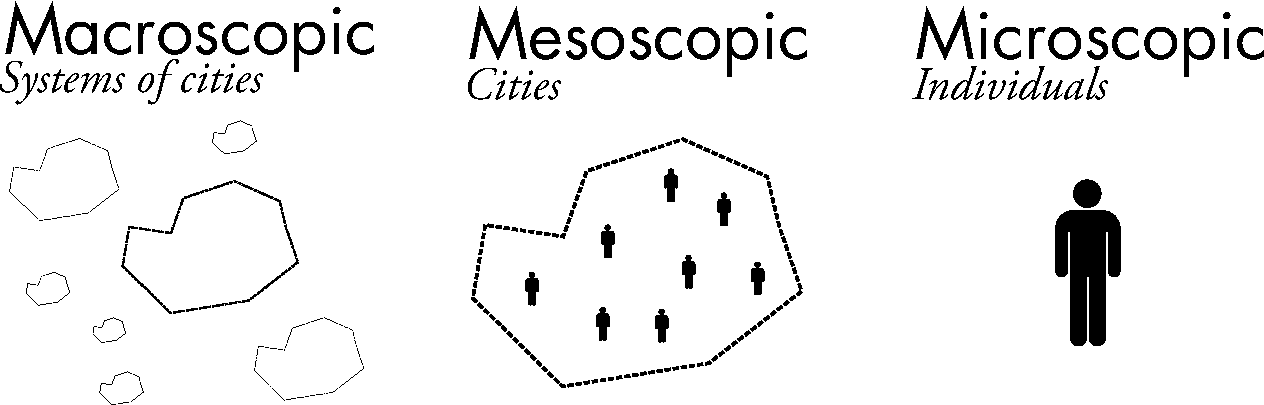
\includegraphics[width=\textwidth]{./gfx/chapter-intro/spatial_scales.pdf}
    \caption{{\bf Interactions at different spatial scales.} Cities are the
    result of interactions occuring at different spatial scales. The movement
and interactions of individuals result in the properties of the city as a whole.
But cities are not closed systems, and interact with other cities in a system of
cities.\label{fig:spatialscale}}
\end{figure}


Cities are therefore the result of interactions occuring at different spatial
scales. Furthermore, they are not static: they evolve in time, through various
processes taking place at different time scales.



\subsection{Time scales}
\label{ssub:time_scales}

First we have time scales of the order of a day, which span the daily commuting
of inhabitants. This incessant movement of people has been traditionally
explored through surveys, but new data now allow more thorough studies. The
digital traces that are left by people at all times (through their mobile phone,
metro pass or GPS device) indeed allow us to explore the structure of flows and
the pace of life in cities at unprecedently fine spatial and time resolutions.

Then, at the order of a year one can see the variation in terms of wealth,
population, etc. of cities, as recorded by statistical agencies. Data about
demographic, social and economic aspects of urban systems allow us to
characterise more specifically the structure and behaviour of these systems.

Finally, at time scales of the order of a decade, we can see the city's
infrastructure as well as its spatial footprint evolve. The study of the
underlying processes is made possible by various projects lead by the GIS
community, historians and geographers which aim at digitizing historical maps of
the road and rail networks in different regions of the world. Also, since the
$1970s$, many satellites have been taking pictures of the Earth's surface, and
the remote sensing community has been treating these data to get information
about the spatial extension of cities. These data should give us some insight
about the processes responsible for the long-term evolution of cities'
structure.\\

\begin{figure}[!h]
    \centering
    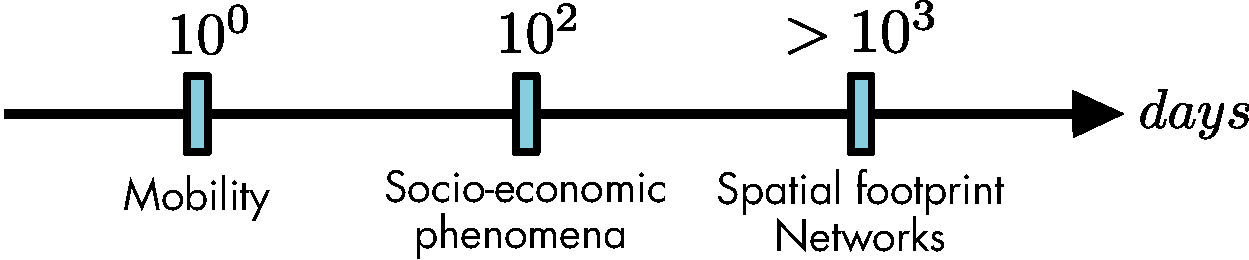
\includegraphics[width=0.9\textwidth]{./gfx/chapter-intro/time_scales.pdf}
    \caption{{\bf Different time scales.} The various data available about
    cities are associated with different time scales.\label{fig:timescale}}
\end{figure}

These time scales are summarised on Fig.~\ref{fig:timescale}. The long-term goal
of our studies is to understand exactly how cities and systems of cities behave,
and how interactions between these three layers lead to the behaviours we
observe. 
